\section{MIMO in handsets} % (fold)
\label{sec:mimo_in_handsets}
Multiple-input and multiple-output (MIMO) is a effective way of dealing with the challenges in delivering more throughput and coupe with the multipath effects from buildings etc. The purpose of this section is to explain what is understood by such a system, how it relates to the antenna design and how it makes a difference. The principal mechanisms and performance metrics are explained. This section will not describe the statistical channel models, but rather focus on the antenna related perspectives. 

\begin{figure}[htbp]
  \centering
  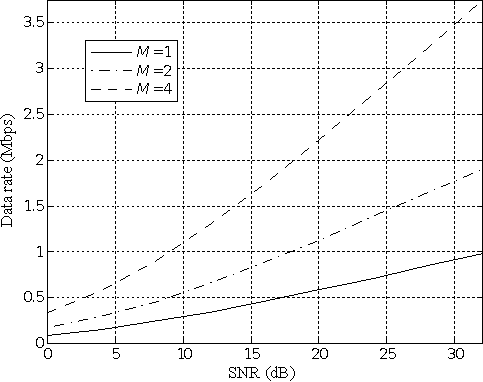
\includegraphics[scale=1.2]{img/analysis/datarateMimo}
  \caption{Throughput versus SNR given a specific M-ary MIMO-setup\cite{Ezio2007MIMO}}
  \label{fig:mimo-throughput}
\end{figure}

\subsection{Perks of MIMO} 
As shown in the introduction to this section, the use of MIMO comes with enhancement in performance. Figure~\ref{fig:mimo-throughput} showed the general performance increase, however this is gained by the addition of multiple different performance gains. The performance gains are spatial diversity gain, multiplexing gain, array gain and interference reduction\cite{Ezio2007MIMO}, which will be described briefly in the following.

\subsubsection{Spatial Diversity Gain}
The spatial diversity gain, improves the resistance to fading in the receiver. This is done by providing the receiver with multiple different copies of the same transmitted signal, ideally the copies are independent from another. A diversity technique is required to combine the signals at the receiver\cite{Ezio2007MIMO}, some examples could be equal gain combining, maximal-ratio combining or selection combining. The spatial diversity is also quite intuitive since the probability that one of the signals are not in a fade increases per added element, given that they are somewhat independent. 
 
\subsubsection{Spatial Multiplexing Gain}
Spatial multiplexing can be used in scatter rich channels, where each received signal are independent. Instead of transmitting the same signal, as with the diversity gain, the spatial multiplexing transmits multiple independent data stream. This allows for a linear increase in the data rate thus the capacity of the wireless network is increased. Generally the number of independent streams that can be supported are limited by the number of receive antennas. \cite{}

\subsubsection{Array Gain}
The array gain is the result of coherent combining of the wireless signals at the receiver, which results in an increase in the receive SNR. The array gain is improved by the number of antenna elements until a certain saturation point. This gain improves the resistance to noise and thus also the coverage. \cite{} 
  
\subsubsection{Interference Gain}
By using MIMO the interference from different users and base-stations can be avoided by exploiting extra spatial degrees of freedom, such as array gain. Furthermore, beam-steering could be implemented such that the signal could be directed towards the designated receiver. Obviously all of the above can not be used at the same time, however using a combination  allows for improved coverage, capacity and reliability. \cite{}
 
\subsection{Antenna Design in MIMO Applications}
The three most important factors in MIMO antenna design are: near-field coupling, the envelope correlation $\rho_e$ and total efficiency $\eta_{\text{total}}$. The near-field coupling is a measure of the coupled power towards the second antenna when the first antenna is excited. The coupling is evaluated by the $S_{21}$ parameter and is often referred to as the \emph{isolation}. This isolation affects the efficiency and envelope correlation coefficient~\cite{Tatomirescu2011PortIsolation}. 

The total efficiency is simply given by Equation~\ref{eq:mimo_total_eff}\cite{Tatomirescu2011PortIsolation}, where $\eta_{\text{rad}}$ is the radiation efficiency, which takes dielectric and conductive losses into account. 
\begin{align} 
\label{eq:mimo_total_eff}
\eta_{\text{total}}=\eta_{\text{rad}} (1-|S_{11}|^2 - |S_{21}|^2)
\end{align}
In practice, the total efficiency may be found directly by supplying a known amount of power to the antenna and observing the power radiated by the antenna. The total efficiency is then the ratio of the radiated power to the supplied/total power:
\begin{align}
    \label{eq:mimo_total_eff_satimo}
    \eta_{\text{total}} = \frac{P_{\text{rad}}}{P_{\text{total}}}
\end{align}
The radiated power is proportional to the spherical integral of the farfield obtained in an anechoic chamber:
\begin{equation}
    \label{eq:mimo_prad}
    P_{\text{rad}} \propto \intsphere{|F_{\theta}|^2 + |F_{\phi}|^2}
    % P_{\text{rad}} \propto \int_0^{2\pi}\int_0^{\pi} |F_{\theta}|^2 + |F_{\phi}|^2\ \sin{\theta}d\phi d\theta
\end{equation}
where $F$ is the complex field sampled for each polarization. The total power, $P_{\text{total}}$, can be found (relatively) by rearranging Equation~\ref{eq:mimo_total_eff_satimo} and using Equation~\ref{eq:mimo_prad} \emph{on a reference antenna} with known total efficiency, $\eta_{\text{total}}^{\prime}$ (here, $^{\prime}$ denotes the reference antenna):
\begin{equation}
    \label{eq:mimo_ptot}
    P_{\text{total}} \propto \frac{P_{\text{rad}}^{\prime}}{\eta_{\text{total}}^{\prime}}
\end{equation}
As both the radiated power and the total power is now found using the same relative power measure (the same radiated-power formula, Equation~\ref{eq:mimo_prad}), the total efficiency can be found using Equation~\ref{eq:mimo_total_eff_satimo}.

The envelope correlation coefficient can be calculated by Equation~\ref{eq:envlop_corr} \cite{Wang2010}. The far-field radiation pattern, $F$ for each polarization, needs to be measured in order to reliably calculate the envelope correlation coefficient.
\begin{align} 
\label{eq:envlop_corr}
\rho = 
\left|  
%
\frac
{\intsphere{A_{12}(\theta,\phi)}}
{\sqrt{\intsphere{A_{11}(\theta,\phi)} \intsphere{A_{22}(\theta,\phi)}}}
%
\right|^2
\end{align}
where
\def\xpr{\text{XPR}}
\begin{where}
\item[$A_{mn}$]
    $
    \xpr_{mn} \cdot E_{\theta,m}(\theta,\phi) E^*_{\theta,n}(\theta,\phi) P_{\theta}(\theta,\phi)
    +
    E_{\phi,m}(\theta,\phi)E^*_{\phi,n}(\theta,\phi)P_{\phi}(\theta,\phi)
    $
\item[$E_{x,m}(\theta,\phi)$] The recorded complex farfield in the polarization $x$ of antenna $m$.
\item[$P_x(\theta,\phi)$] The distribution of incoming waves for polarization $x$. If the distribution is assumed to be isotropic, this can be set to $1/4\pi$.
\item[$\xpr_{mn}$] Cross polarization ratio $= P_{v,m}/P_{h,n}$ for the antenna set $mn$.
\item[$P_{v,m}$] Relative power in the $\theta$ polarization, 
    \begin{equation*}
        P_v = \intsphere{|E_{\theta,m}|^2}
    \end{equation*}
\item[$P_{h,n}$] Relative power in the $\phi$ polarization,
    \begin{equation*}
        P_h = \intsphere{|E_{\phi,n}|^2}
    \end{equation*}
\end{where}

% \begin{align} 
% \label{eq:envlop_corr}
% \rho = \frac{\oint(\text{XPD} \cdot E_{\theta X}(\Omega) \cdot) E^*_{\theta X} \cdot p_\theta(\Omega)+E_{\phi Y}(\Omega) \cdot) E^*_{\phi Y} \cdot p_\phi(\Omega) )d\Omega}{\sqrt{\oint(\text{XPD}\cdot G_{\theta X}(\Omega) \cdot p_\theta(\Omega)+G_{\phi X}(\Omega) \cdot p_\phi(\Omega))d\Omega \cdot \oint(\text{XPD}\cdot G_{\theta Y}(\Omega) \cdot p_\theta(\Omega)+G_{\phi Y}(\Omega) \cdot p_\phi(\Omega))d\Omega }}
% \end{align}
\fixme{Søren: Write the form used in the actual implementation.}

Equation~\ref{eq:envlop_corr} assumes uniform 3D angular power spectrum of the received signal and is not valid if this is not the case. The envelope correlation coefficient can also be estimated by the S-parameters, as given in Equation~\ref{eq:envlop_corr_Sparams}\cite{Alain2010MIMO}. However, the use of this is often discouraged since it assumes very high radiation efficiency. \cite{}
\begin{align}
\label{eq:envlop_corr_Sparams}
  \rho_e \approx |\rho_c|^2 = \frac{|S^*_{11}S_{12}+S^*_{21}S_{22}|^2}{(1-|S_{11}|^2-|S_{21}|^2)(1-|S_{22}|^2-|S_{12}|^2)}
\end{align}
Thus, when designing antenna for the purpose of MIMO, the antennas need to be designed in a way such that the elements receives de-correlated signals. This can be done in different ways, such as changing the angular patterns, changing the polarization of the elements, or spatially separating the antennas, which are the most used methods. However, there are also other techniques such as decoupling networks, parasitic elements, active antenna cancellation, eigenmodes and balanced currents. 

\fixme{Cites!}

\subsubsection{Spatial Correlation}
The spatial correlation between two antennas is given by the radiated E-field patterns as given in Equation~\ref{eq:envlop_corr}. There it is seen that the correlation is a comparison between the radiated E-field patterns and the incident E-fields arriving at the antenna, which is given by the probability $p_\theta$ and $p_\phi$. 

From the Equation~\ref{eq:envlop_corr} it can also be deduced that the spacing, polarization and radiation patterns effects the correlation between two antennas. In order to investigate the only effects of spacial separation we consider the case with two omnidirectional antennas both vertically polarized. This can be described by Equation~\ref{eqn:spactial_corr}\cite{Tim2012Practical}.
\begin{align}
\label{eqn:spactial_corr}
  \rho = \oint e^{j\beta \sqrt{d^2+l^2}\cos\zeta}p_\theta(\theta,\phi)\sin\theta \, \mathrm{d} \theta \mathrm{d} \phi
\end{align}
\begin{where}
\item[$d$] is the horizontal spacing
\item[$l$] is the vertical spacing
\item[$\cos \zeta$] $= \sin(\phi + \tan^{-1}(l/d)\ \text{sgn}\phi)\sin\phi$   
\end{where}

In Figure~\ref{fig:mimo-spacing}, two cases of Equation~\ref{eqn:spactial_corr} are shown, one where only the horizontal spacing is considered and another where only the vertical spacing is considered. The angle of arrival is given by Taga\fixme{elaborate on the angle of arrival}, where the mean angle $\overline{\theta}$ is at \SI{70}{\degree} and the standard deviation $\sigma_\theta$ is \SI{20}{\degree}. From the plot it can be seen that the vertical spacing required for a certain correlation is larger than that of the horizontal spacing. This comes from the Taga-model used for the angle of arrival, since its distribution is nonuniform. This can however not be used to argue that the antennas should be spaced horizontally, since smartphones often is operated both horizontally and vertically. 

It is also possible to make the array in other topologies such as planar, circular or random. This is, however, not very practical for mobile devices given the current usage of low frequencies in telecommunication (\SIrange{500}{2700}{MHz}) as described in Section~\ref{sec:lte}.

\begin{figure}[htbp]
  \centering
  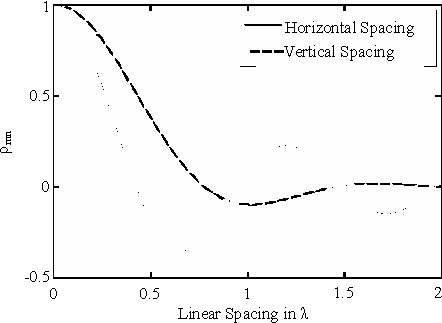
\includegraphics[scale=1.2]{img/analysis/mimoSpacing}
  \caption{Spacing versus wavelength for the horizontal and vertical case\cite{Tim2012Practical}}
  \label{fig:mimo-spacing}
\end{figure}

\subsubsection{Polarization and Radiation Patterns}
In addition to the spatial separation to decorrelate antennas, polarization and different radiation patterns can also be used to decorrelate elements. This is very often used in small mobile devices, where the physical size limits the spacing between elements.  

In theory, using a perfectly polarized dipole and loop antenna, it would be possible to create total decorrelated elements, because they have opposite polarization. This is obviously hard to implement in practice, but it is possible to lower the correlation of to elements by having a difference in polarization. However, using different polarization to get a lower correlation requires a suitable XPR in the channel. The XPR should be around \SI{6}{dB} or lower\cite{Tim2012Practical}. 

\subsubsection{Multiplexing Efficiency}
\fixme{Søren: Write about multiplexing efficiency.}

Multiplexing efficiency is a measure of total efficiency for an antenna system, taking into account the total efficiency for each antenna \emph{and} the correlation between antenna elements. In this way, it is a single parameter that describes the total loss in SNR (or power) when using a MIMO antenna system \cite{tian2011multiplexing}.

For a $2\times2$ MIMO system, relevant to this project, and assuming high SNR, the multiplexing efficiency, $\eta_{\text{mux}}$, is computed as \cite{tian2011multiplexing}
\begin{equation}
    \eta_{\text{mux}} = \sqrt{\eta_1 \eta_2 (1 - |\rho|^2)}
\end{equation}
where
\begin{where}
\item[$\eta_n$] Total efficiency of the $n$th antenna.
\item[$\rho$] Correlation between antenna 1 and 2.
\end{where}

In the rest of the report, efficiency and correlation will mostly be teated separately to see more details between the antennas. However, the metric of multiplexing may be useful when evaluating the antennas performance in a link budget.
